\documentclass{beamer}
\usetheme{Madrid}

\usepackage{amsmath, amssymb, amsthm}
\usepackage{graphicx}
\usepackage{gensymb}
\usepackage[utf8]{inputenc}
\usepackage{hyperref}
\usepackage{tikz}


\title{2.6.12 }
\author{AI25BTECH11006 - Nikhila}
\date{31-08-2025}

\begin{document}

\frame{\titlepage}

% Question frame
\begin{frame}
\frametitle{Question}
Find the sine of the angle between the vectors $\textbf{a} = 3\hat{i} + \hat{j} + 2\hat{k}$ and $\textbf{b} = 2\hat{i} + -2\hat{j} + 4\hat{k}$.\\
 \end{frame}




% Solution steps
\begin{frame}
\frametitle{Solution}
The given vectors are $\vec{a}\begin{pmatrix}3 \\ 1 \\ 2\end{pmatrix} $ and $  \vec{b}\begin{pmatrix}2 \\ -2 \\ 4\end{pmatrix}$ \\ 

We know that
\begin{align}
\cos\theta = \frac{\vec{a}^T \vec{b}}{\lVert \vec{a} \rVert \hspace{0.3em} \lVert \vec{b} \rVert}
\end{align}

and

\begin{align}
\sin\theta = \sqrt{1 - \cos^2\theta}
\end{align}

\begin{align}
\vec{a}^T \vec{b} &= 3(2) + 1(-2) + 2(4) = 6 - 2 + 8 = 12
\end{align}

\end{frame}


\begin{frame}
\frametitle{Solution}

\begin{align}
\lVert \vec{a} \rVert &= \sqrt{(3)^2 + (1)^2 + (2)^2} = \sqrt{14}, \\
\lVert \vec{b} \rVert &= \sqrt{(2)^2 + (-2)^2 + (4)^2} = \sqrt{24}.
\end{align}

\begin{align}
\cos\theta &= \frac{12}{\sqrt{14} \cdot \sqrt{24}} \\
&= \frac{12}{\sqrt{336}} \\
&= \frac{\sqrt{3}}{\sqrt{7}}
\end{align}

\end{frame}

\begin{frame}
\frametitle{Solution}

\begin{align}
\sin\theta &= \sqrt{1 - \left(\frac{\sqrt{3}}{\sqrt{7}}\right)^2} \\
&= \sqrt{1 - \frac{3}{7}} \\
&= \frac{2}{\sqrt{7}}
\end{align}

\end{frame}


% Graphical representation
\begin{frame}
\frametitle{Graphical Representation}
\begin{center}
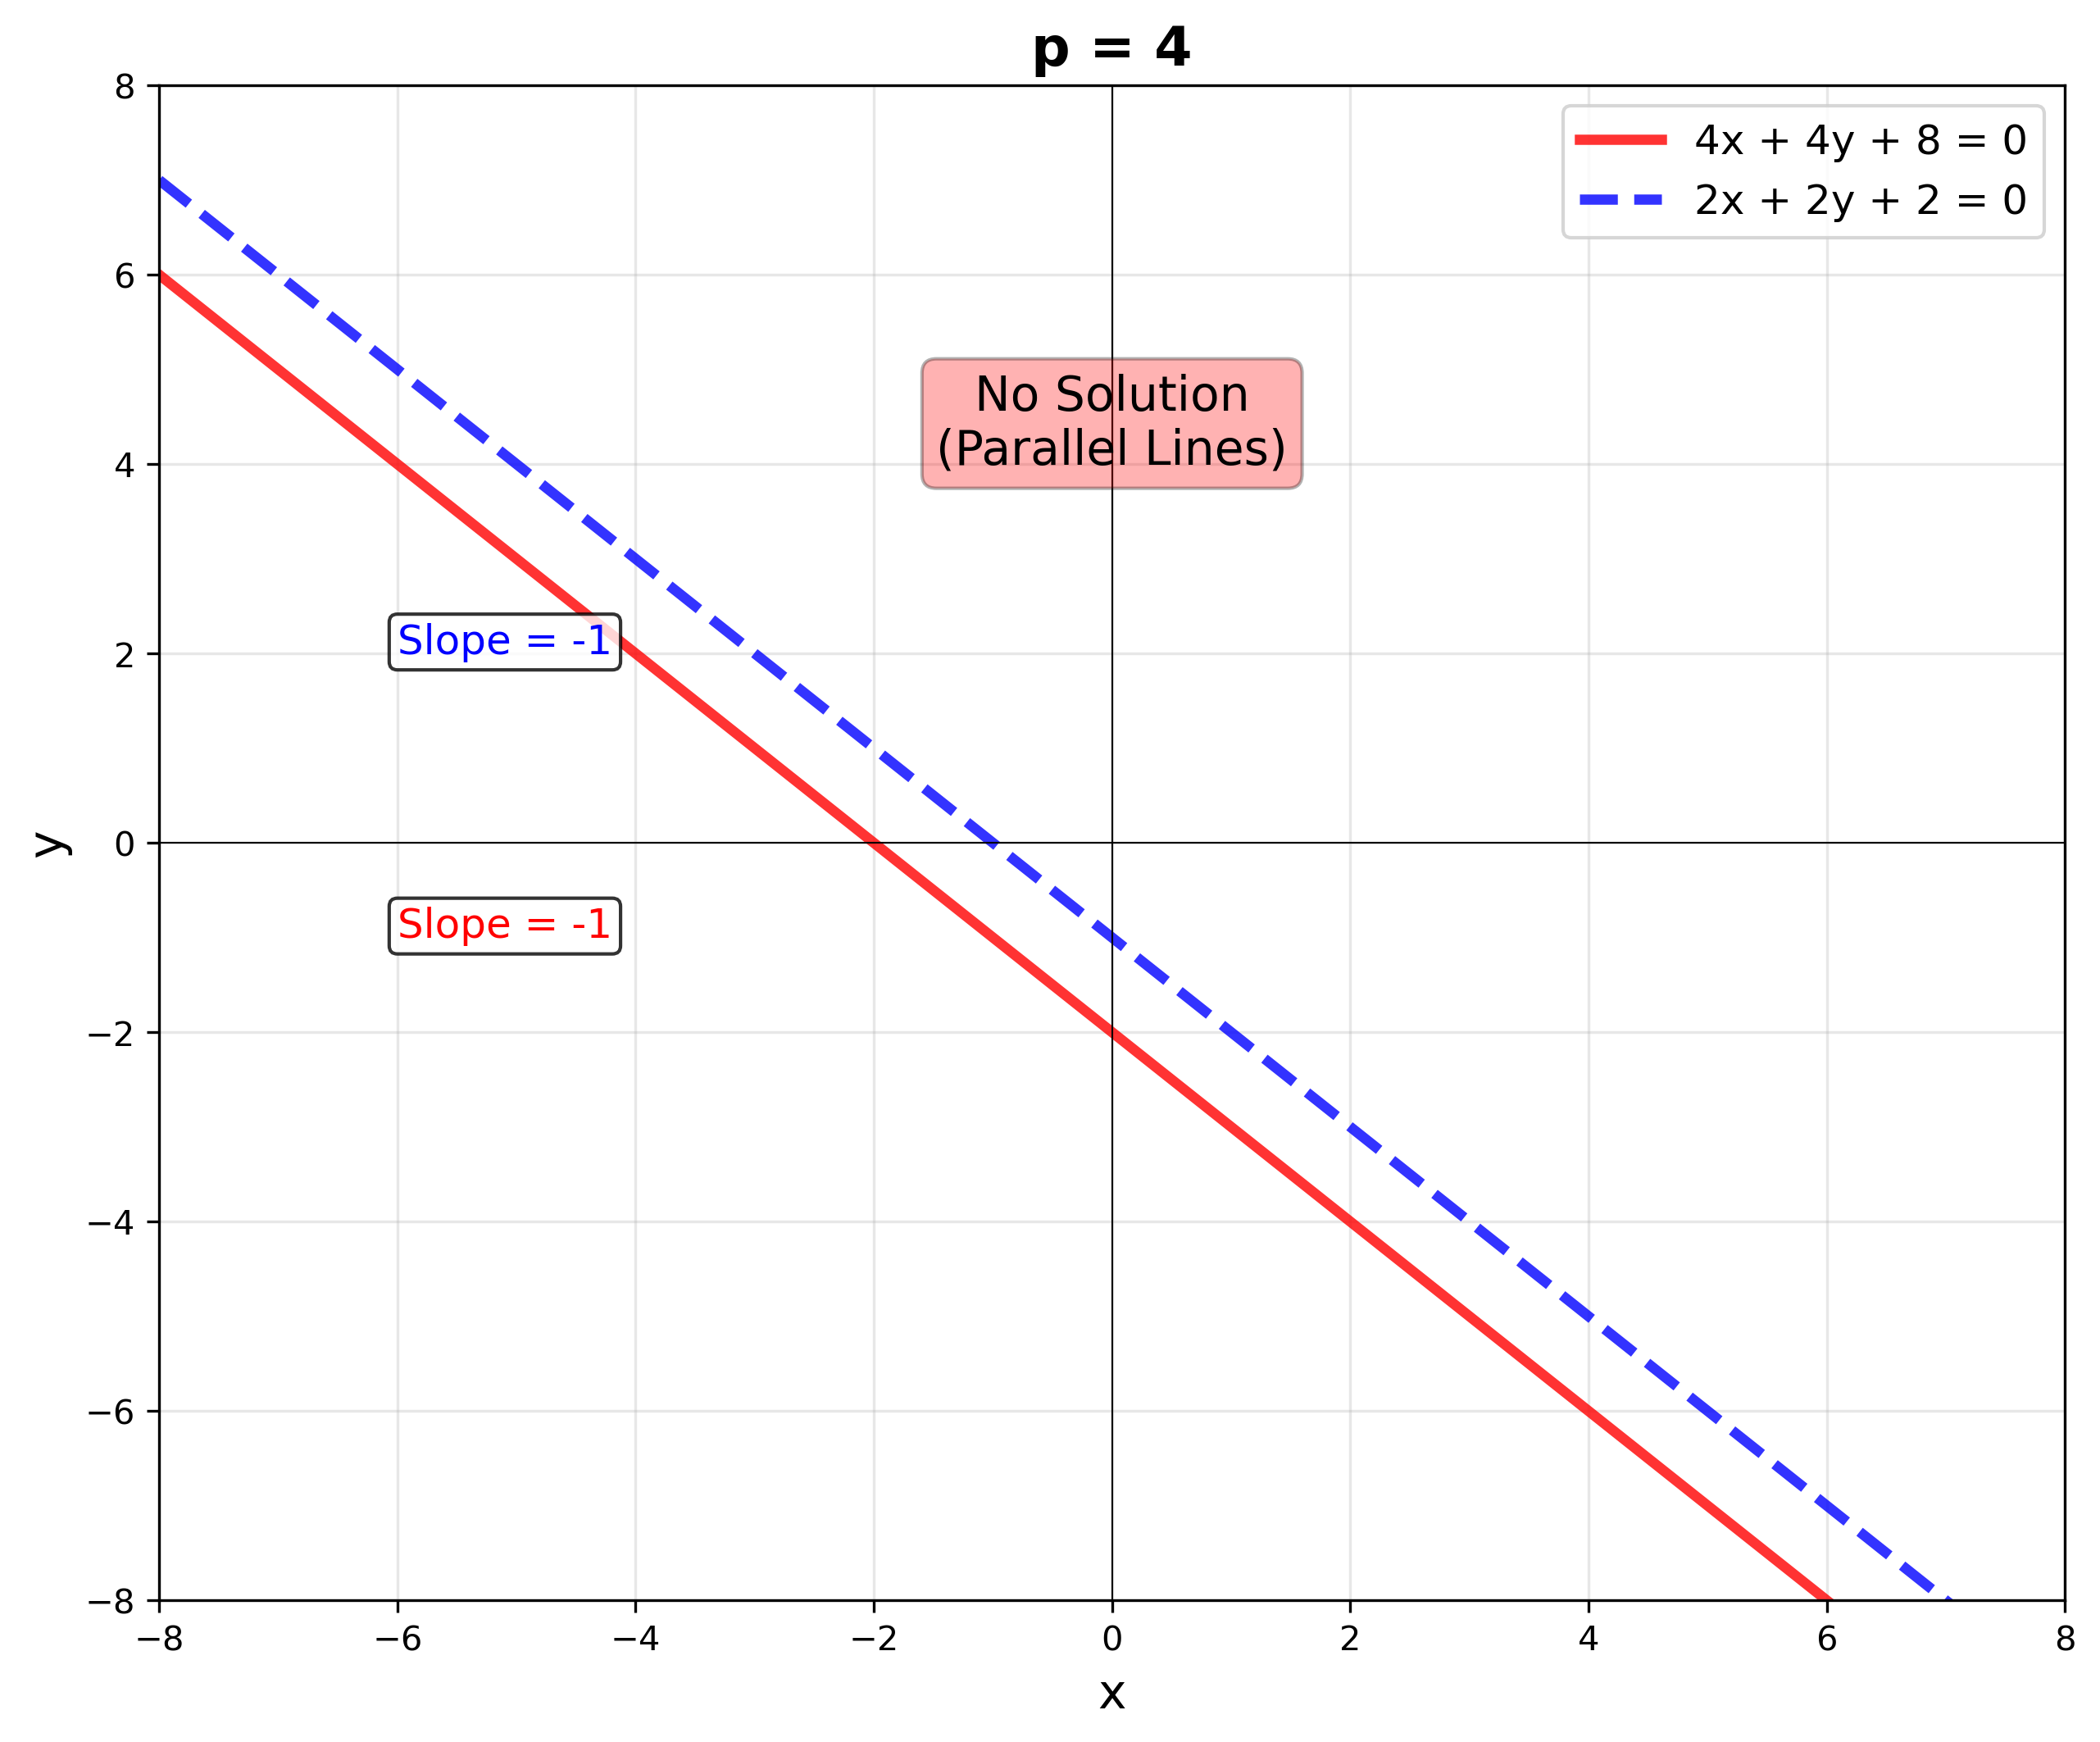
\includegraphics[width=0.8\linewidth]{fig1.png}
\end{center}
\end{frame}

\end{document}

